\documentclass[10pt,a4paper]{article}
\usepackage{amsmath,amssymb,amsthm,graphicx}
\usepackage{amsmath,amssymb,amsfonts,amsthm,mathtools,graphicx}
\usepackage[dvipsnames,svgnames,table]{xcolor}
\usepackage{hyperref}
\usepackage{braket,thmtools,thm-restate,tikz,wrapfig}
\allowdisplaybreaks
\newtheorem{theorem}{Theorem}
%

\newtheorem{lemma}[theorem]{Lemma}
\newtheorem{proposition}[theorem]{Proposition}
\newtheorem{corollary}[theorem]{Corollary}
\newtheorem{definition}[theorem]{Definition}
\newtheorem{conjecture}[theorem]{Conjecture}
\newtheorem{fact}[theorem]{Fact}
\newtheorem{open}{Open Problem}
\theoremstyle{definition}

\newenvironment{namedtheorem}[2]
	{\begin{trivlist}\item {\bf #1} (#2){\bf .}\em}{\end{trivlist}}

%
%
%
%

\newcommand{\eq}[1]{\hyperref[eq:#1]{(\ref*{eq:#1})}}
\renewcommand{\sec}[1]{\hyperref[sec:#1]{Section~\ref*{sec:#1}}}
\newcommand{\thm}[1]{\hyperref[thm:#1]{Theorem~\ref*{thm:#1}}}
\newcommand{\lem}[1]{\hyperref[lem:#1]{Lemma~\ref*{lem:#1}}}
\newcommand{\defn}[1]{\hyperref[def:#1]{Definition~\ref*{def:#1}}}
\newcommand{\prop}[1]{\hyperref[prop:#1]{Proposition~\ref*{prop:#1}}}
\newcommand{\cor}[1]{\hyperref[cor:#1]{Corollary~\ref*{cor:#1}}}
\newcommand{\fig}[1]{\hyperref[fig:#1]{Figure~\ref*{fig:#1}}}
\newcommand{\tab}[1]{\hyperref[tab:#1]{Table~\ref*{tab:#1}}}
\newcommand{\alg}[1]{\hyperref[alg:#1]{Algorithm~\ref*{alg:#1}}}
\newcommand{\app}[1]{\hyperref[app:#1]{Appendix~\ref*{app:#1}}}
\newcommand{\conj}[1]{\hyperref[conj:#1]{Conjecture~\ref*{conj:#1}}}
\newcommand{\chap}[1]{\hyperref[chap:#1]{Chapter~\ref*{chap:#1}}}
\newcommand{\fct}[1]{\hyperref[fct:#1]{Fact~\ref*{fct:#1}}}
\DeclareMathOperator{\poly}{poly}
\DeclareMathOperator{\polylog}{polylog}
\newcommand{\tO}{\tilde{O}}
\newcommand{\tOmega}{\tilde{\Omega}}
\newcommand{\tTheta}{\widetilde{\Theta}}

%
%
%
%

\DeclareMathOperator{\Dom}{Dom}

\newcommand{\B}{\{0,1\}}
\newcommand{\Ba}{\{0,1,*\}}
\newcommand{\Bao}{\{0,1,*,\dagger\}}
\newcommand{\Bo}{\{0,1,\dagger\}}

\newcommand{\X}{\mathcal{X}}
\newcommand{\Y}{\mathcal{Y}}
\newcommand{\Z}{\mathcal{Z}}
\newcommand{\CC}{\textsc{CC}}

%
%
%
%

% Unused custom blackboard alphabet omitted.

\renewcommand{\>}{\rangle}
\newcommand{\<}{\langle}
\DeclareMathOperator{\Tr}{Tr}
%
\newcommand{\id}{\mathbf{1}}
\DeclareMathOperator*{\E}{\mathbb{E}} 
\DeclareMathOperator{\bR}{\mathbb{R}}
\DeclareMathOperator{\bN}{\mathbb{N}}
\DeclareMathOperator{\re}{Re}
\DeclareMathOperator{\supp}{supp}
\DeclareMathOperator{\Out}{\mathcal{O}}
\newcommand{\cB}{\mathcal{B}}
\newcommand{\fh}{\mathfrak{h}}
\newcommand{\tX}{\widetilde{X}}
\newcommand{\tY}{\widetilde{Y}}

\newcommand{\tth}[1]{$#1^\mathrm{th}$}
\newcommand{\cl}[1]{\mathsf{#1}}
\newcommand{\norm}[1]{{\left\lVert#1\right\rVert}}

%
%
%
%

\newcommand{\OR}{\textsc{OR}}
\newcommand{\PrOR}{\textsc{PrOR}}
\newcommand{\AND}{\textsc{AND}}
\newcommand{\MAJ}{\textsc{MAJ}}
\newcommand{\BSum}{\textsc{BSum}}
\newcommand{\BKK}{\textsc{BKK}}
\newcommand{\Ind}{\textsc{Ind}}
\newcommand{\NAND}{\textsc{Nand}}
\newcommand{\ANDOR}{\textsc{And-Or}}
\newcommand{\PARITY}{\textsc{Parity}}
\newcommand{\ksum}{k\textsc{-sum}}
\newcommand{\Simon}{\textsc{Simon}}
\newcommand{\NANDtree}{\textsc{NAND-tree}}
\newcommand{\Disj}{\textsc{Disj}}
\newcommand{\IP}{\textsc{IP}}
\newcommand{\XOR}{\textsc{XOR}}
\newcommand{\triv}{\textsc{triv}}

%
%
%
%

\DeclareMathOperator{\D}{D}
\DeclareMathOperator{\R}{R}
\DeclareMathOperator{\Q}{Q}
\DeclareMathOperator{\C}{C}
\DeclareMathOperator{\UC}{UC}
\DeclareMathOperator{\RC}{RC}
\DeclareMathOperator{\RS}{RS}
\DeclareMathOperator{\DS}{DS}
\DeclareMathOperator{\QS}{QS}
\DeclareMathOperator{\QC}{QC}
\DeclareMathOperator{\s}{s}
\DeclareMathOperator{\bs}{bs}
\DeclareMathOperator{\fbs}{fbs}
\DeclareMathOperator{\cbs}{cbs}
\DeclareMathOperator{\cfbs}{cfbs}
\DeclareMathOperator{\Adv}{Adv}
\DeclareMathOperator{\prt}{prt}
\newcommand{\UCmin}{\UC_{\min}}
\DeclareMathOperator{\M}{M} 
\DeclareMathOperator{\CAdv}{CAdv}
\DeclareMathOperator{\RCC}{RCC}
\DeclareMathOperator{\QCC}{QCC}
\DeclareMathOperator{\sAdv}{sAdv}
\DeclareMathOperator{\QICZ}{QICZ}
\DeclareMathOperator{\IC}{IC}
\DeclareMathOperator{\QIC}{QIC}
\DeclareMathOperator{\CIC}{CIC}
\DeclareMathOperator{\HQIC}{HQIC}
\DeclareMathOperator{\crit}{crit}
\DeclareMathOperator{\bias}{bias}
\DeclareMathOperator{\info}{info}

%
\DeclareMathOperator{\ndeg}{ndeg}
\DeclareMathOperator{\avdeg}{avdeg}
\DeclareMathOperator{\adeg}{\widetilde{\deg}}
\DeclareMathOperator{\aavdeg}{\widetilde{\avdeg}}
\newcommand{\degp}{\deg^{+}}
\newcommand{\degpmin}{\deg^{+}_{\min}}
\newcommand{\adegp}[1]{\adeg^{+#1}}
\newcommand{\adegpmin}[1]{\adeg^{+#1}_{\min}}
\newcommand{\avdegp}{\avdeg^{+}}
\newcommand{\avdegpmin}{\avdeg^{+}_{\min}}
\newcommand{\aavdegp}[1]{\aavdeg^{+#1}}
\newcommand{\aavdegpmin}[1]{\aavdeg^{+#1}_{\min}}

%
%
\title{Classical adversary bounds lift to randomized communication complexity with a constant-size versatile gadget}
\author{Anurag Anshu, Shalev Ben-David, Srijita Kundu}
\date{doi:10.4230/LIPIcs.CCC.2021.30; CC BY 4.0}
\begin{document}
\maketitle
\noindent\textit{Editorial note.} Editable transcription of corresponding formally published CC BY classical lifting statement/proof, using nonexclusive native only as private aid. Public body blanks all excluded native ranges and comments while preserving locator lines; no whole unselected native file is publicly referenced. Author math macros flattened without input/include; unused custom bbold alphabet omitted. Native global theorem offset restored for selected background, and comparison mentions of omitted query-relations chapter rendered as accurate originalSection6. Quantum conditional lifting and separate query-relation proofs not imported into this classical record. All production/extraction/validation solely on Yupeng; no local compilation.\par\medskip
\noindent\textit{Allowed standard prerequisites (editorial).}\begin{itemize}
\item Randomized communication with public randomness, classical adversary weight schemes, Hellinger distance and conditional information identities. Complete originalSection2 models/measure definitions and standard cited information facts retained; source-local versatile gadget/sampling and complete lifting proof included
\end{itemize}\medskip
\begin{theorem}[Original Theorem 1]\label{thm:CAdv_lift}
There is an explicitly given function $G:\X\times\Y\to\B$ such that for any (possibly partial) Boolean function or relation $f$,
\[\RCC(f\circ G)=\Omega(\CAdv(f)).\]
\end{theorem}
Here $\RCC(f\circ G)$ denotes the randomized communication complexity of $f\circ G$ with shared randomness.

\setcounter{section}{1}\setcounter{theorem}{8}\section{Preliminaries}
\subsection{Distance \& information measures}
We define all the distance and information measures for quantum states. The classical versions can be obtained by making the corresponding registers classical.

The $\ell_1$ distance between two quantum states $\rho$ and $\sigma$ is defined as
\[ \norm{\rho-\sigma}_1 = \Tr\sqrt{(\rho-\sigma)^\dagger(\rho-\sigma)}.\]

The entropy of a quantum state $\rho_A$ on register $A$ is defined as
\[H(A)_\rho = -\Tr(\rho\log\rho).\]
For a state $\rho_{AB}$ on registers $AB$, the conditional entropy of $A$ given $B$ is
\[ H(A|B)_\rho = H(AB)_\rho - H(B)_\rho.\]
Conditional entropy satisfies the following continuity bound \cite{AF04}: if $\rho$ and $\sigma$ on registers $AB$ satisfy $\norm{\rho-\sigma}_1 \leq \epsilon$, then
\[ |H(A|B)_\rho - H(A|B)_\sigma| \leq 4\epsilon\log|A| + 2h(\epsilon) \]
where $h(.)$ is the binary entropy function.
For $\rho_{ABC}$, we define the mutual information and conditional mutual information as
\[ I(A:B)_\rho = H(A)_\rho - H(A|B)_\rho \qquad I(A:B|C) = H(A|C)_\rho - H(A|BC)_\rho. \]
Mutual information satisfies
\[ 0 \leq I(A:B|C)_\rho \leq \min\{\log|A|,\log|B|\}\]
and the chain rule
\[ I(A:BC)_\rho = I(A:B)_\rho + I(A:C|B)_\rho.\]


\subsection{Query complexity}\label{sec:prelim_query}

In query complexity, the primary object of study
are Boolean functions, which are functions
$f\colon\B^n\to\B$ where $n$ is a positive integer. Often,
we will actually study partial Boolean functions, which
are defined on only a subset of $\B^n$. We will use
$\Dom(f)$ to denote the domain of $f$; this is a subset
of $\B^n$.

For a (possibly partial) Boolean function $f$, we use
$\D(f)$, $\R(f)$, and $\Q(f)$ to denote its deterministic
query complexity, randomized query complexity (to bounded error),
and quantum query complexity (to bounded error), respectively.
For the definition of these measures, see \cite{BdW02},
though we won't use these definitions in this work.

\subsubsection{Block sensitivity and its variants}

We will use the following definitions.

\paragraph{Block notation.} For a Boolean string $x\in\B^n$
and a set $B\subseteq[n]$, we let $x^B$ denote the
string with the bits in $B$ flipped; that is,
$x^B_i=x_i$ for all $i\notin B$ and $x^B_i=1-x_i$ for all $i\in B$.
The set $B$ is called a \emph{block}.

\paragraph{Sensitive block.} For a (possibly partial) Boolean
function $f$ on $n$ bits and an input $x\in\Dom(f)$, we say that
a set $B\subseteq[n]$ is a \emph{sensitive block} for $x$
(with respect to $f$) if $x^B\in\Dom(f)$ and $f(x^B)\ne f(x)$.

\paragraph{Block sensitivity.} The \emph{block sensitivity}
of a string $x\in\B^n$ with respect to a (possibly partial)
Boolean function $f$ satisfying $x\in\Dom(f)$ is the maximum
integer $k$ such that there are $k$ blocks
$B_1,B_2,\dots,B_k\subseteq[n]$ which are all sensitive
for $x$ and which are all disjoint. This is denoted
$\bs(x,f)$.

\paragraph{Block sensitivity of a function.} The
\emph{block sensitivity} of a (possibly partial) Boolean function
$f$ is the maximum value of $\bs(x,f)$ over $x\in\Dom(f)$.
This is denoted $\bs(f)$.
Block sensitivity was originally introduced by Nisan
\cite{Nis91}, and is discussed in the survey by Buhrman and
de Wolf \cite{BdW02}.

\paragraph{Fractional block sensitivity.} The
\emph{fractional block sensitivity} of a string $x\in\B^n$
with respect to a (possibly partial) Boolean function $f$
satisfying $x\in\Dom(f)$ is the maximum possible
sum of weights $\sum_B w_B$, where the weights $w_B\ge 0$
are assigned to each sensitive block of $x$ and must satisfy
$\sum_{B:i\in B} w_B\le 1$ for all $i\in[n]$.
This is denoted by $\fbs(x,f)$. The fractional block sensitivity
of a function $f$, denoted $\fbs(f)$, is the maximum value of
$\fbs(x,f)$ over $x\in\Dom(f)$.
Fractional block sensitivity was defined by \cite{Aar08},
but see also \cite{KT16}.

\paragraph{Critical block sensitivity.}
For a (possibly partial) Boolean function $f$, we say that
a total Boolean function $f'$ is a \emph{completion} of $f$
if $f'(x)=f(x)$ for all $x\in\Dom(f)$. The \emph{critical block
sensitivity} of $f$, denoted $\cbs(f)$, is defined as
\[\min_{f'}\max_{x\in\Dom(f)}\bs(x,f'),\]
where the minimum is taken over completions $f'$ of $f$.
This measure was defined by \cite{HN12}. It equals $\bs(f)$
for total functions, but may be larger for partial functions.

\paragraph{Critical fractional block sensitivity.}
For a (possibly partial) Boolean function $f$, we define
its \emph{critical fractional block sensitivity}, denoted
$\cfbs(f)$, as
\[\min_{f'}\max_{x\in\Dom(f)}\cfbs(x,f'),\]
where the minimum is taken over completions $f'$ of $f$.
This measure has not previously appeared in the literature.

\subsubsection{Adversary bounds}
\label{sec:prelim_adv}

\paragraph{Positive adversary bound.}
For a (possibly partial) Boolean function $f$,
we define the positive-weight adversary bound,
denoted $\Adv(f)$, as the minimum of the following program.
We will have one non-negative weight $q(x,i)$
for each $x\in\Dom(f)$ and each $i\in[n]$. We call
such a weight scheme feasible if, for all
$x,y\in\Dom(f)$ with $f(x)\ne f(y)$,
we have
\[\sum_{i:x_i\ne y_i} \sqrt{q(x,i)q(y,i)}\ge 1.\]
Then $\Adv(f)$ is defined as the minimum
of $\max_{x\in\Dom(f)}\sum_{i\in[n]} q(x,i)$
over feasible weight schemes $q(\cdot,\cdot)$.
A different version of the positive-weight
adversary bound was defined in \cite{Amb02},
though the version we've currently defined
appears in \cite{LM08} and \cite{SS06}
(in the latter, our definition is equivalent
to $\operatorname{MM}(f)$).

\paragraph{Classical adversary bound.}
For a (possibly partial) Boolean function $f$,
we define the classical adversary bound,
denoted $\CAdv(f)$, as the minimum of the following
program. We will have one non-negative
weight $q(x,i)$ for each $x\in\Dom(f)$ and each $i\in[n]$,
as before. We call such a weight scheme feasible
if, for all $x,y\in\Dom(f)$ with $f(x)\ne f(y)$,
we have
\[\sum_{i:x_i\ne y_i}\min\{q(x,i),q(y,i)\}\ge 1.\]
Then $\CAdv(f)$ is defined as the minimum
of $\max_{x\in\Dom(f)}\sum_{i\in[n]} q(x,i)$
over feasible weight schemes $q(\cdot,\cdot)$.
Observe that this definition is the same as
that of $\Adv(f)$, except that the feasibility
constraint sums up the minimum of $q(x,i)$ and
$q(y,i)$ instead of the geometric mean. This feasibility
constraint is harder to satisfy, and hence we have
$\CAdv(f)\ge\Adv(f)$.
A different version of the classical adversary
was defined in \cite{Aar06}, though the version
we've currently defined appears in \cite{LM08}
and \cite{AKPV18} (in the latter, our definition
is equivalent to $\operatorname{CMM}(f)$).

\paragraph{Singleton adversary bound.}
\cite{ABK+20} introduced a simplified version
of the quantum adversary bound, which we denote
$\Adv_1(f)$. As in the other adversaries,
this will be the minimum over a program that has
one non-negative weight $q(x,i)$ for each pair
of input $x\in\Dom(f)$ and index $i\in[n]$.
The objective value will once again be
$\max_{x\in\Dom(f)}\sum_{i\in[n]} q(x,i)$.
The only difference is the constraints:
instead of placing a constraint
for each $x,y\in\Dom(f)$ with $f(x)\ne f(y)$,
we only place this constraint for such $x,y$
that have Hamming distance exactly $1$.
Observe that this is a relaxation
of the constraint in the definition of $\Adv(f)$,
and hence $\Adv_1(f)\le \Adv(f)$ for all (possibly partial)
Boolean functions $f$.

\subsection{A generalization to relations}

So far, we've defined our query measures for partial
Boolean functions. However, in many cases we will be interested
in studying \emph{relations}, which are a generalization
of partial Boolean functions.

In query complexity, a \emph{relation} is a subset
of $\B^n\times \Sigma$, where $\Sigma$ is some finite
output alphabet. We will equate a relation
$f\subseteq \B^n\times\Sigma$ with a function
that maps $\B^n$ to subsets of $\Sigma$, so that
for a string $x\in\B^n$, the notation $f(x)$ denotes
$\{\sigma\in\Sigma:(x,\sigma)\in f\}$.
An algorithm which computes a relation $f$ to error
$\epsilon$ must have the guarantee that for inputs $x\in\B^n$,
the algorithm outputs a symbol in $f(x)$ with probability
at least $1-\epsilon$.

Relations are generalizations of partial functions.
This is because we can represent a partial function
$f$ with domain $\Dom(f)\subseteq\B^n$ by a relation
$f'$ such that $f'(x)=\{f(x)\}$ for $x\in\Dom(f)$
and $f'(x)=\{0,1\}$ for $x\notin\Dom(f)$. In other words,
the relational version $f'$ of the partial function $f$
will accept all input strings (it will be a total function),
but it will consider every output symbol to be valid
when given an input not in $\Dom(f)$. This essentially
makes the inputs not in $\Dom(f)$ become trivial, and hence
makes the relation $f'$ intuitively equivalent to the partial
function $f$.

We will generalize several of our query measures to relations.

\paragraph{Critical (fractional) block sensitivity.}
The original definition of $\cbs(f)$ from \cite{HN12} actually
defined it for relations.
We say that a total function $f'\colon\B^n\to\Sigma$
is a \emph{completion} of a relation $f\subseteq \B^n\times\Sigma$
if $(x,f'(x))\in f$ for all $x\in\B^n$. In other words,
$f'$ is a completion if it gives a fixed, valid
output choice for each input to $f$. Next, we say an input
$x\in\B^n$ is \emph{critical} if it has a unique valid
output symbol in $f$; that is, if $|f(x)|=1$.
We let $\crit(f)$ denote the set of all critical inputs
to $f$.
(Note that if $f$ is the relational version of a partial function,
then $\crit(f)$ is equal to the domain of the partial function.)
We then define
\[\cbs(f)\coloneqq \min_{f'}\max_{x\in\crit(f)}\bs(x,f')\]
\[\cfbs(f)\coloneqq \min_{f'}\max_{x\in\crit(f)}\fbs(x,f'),\]
where the minimizations are over completions $f'$ of $f$.
Observe that if $f$ is the relational version
of a partial function, these definitions
match the previous ones.

\paragraph{Adversary bounds.}
The adversary bounds easily generalize to relations:
both the positive adversary bound and the classical adversary
bound will still be minimizations over weight schemes
$q(x,i)$, with a non-negative weight assigned to each pair of
input in $\B^n$ and $i\in[n]$. The objective value to be
minimized is the same as before:
$\max_{x\in\B^n}\sum_{i\in[n]} q(x,i)$.
As for the constraints, we previously had one constraint
for each pair of inputs $x,y$ with $f(x)\ne f(y)$.
For relations, we will replace this condition with the condition
$f(x)\cap f(y)=\varnothing$ (that is, $x$ and $y$ have
disjoint allowed-output-symbol sets). Hence the new constraint
for $\Adv(f)$ becomes that for all pairs $x,y\in\B^n$
with $f(x)\cap f(y)=\varnothing$, we have
\[\sum_{i:x_i\ne y_i}\sqrt{q(x,i)q(y,i)}\ge 1.\]
Similarly, the constraint for $\CAdv(f)$ is that for all pairs
$x,y\in\B^n$ with $f(x)\cap f(y)=\varnothing$, we have
\[\sum_{i:x_i\ne y_i}\min\{q(x,i),q(y,i)\}\ge 1,\]
and the constraint for $\Adv_1(f)$ is similar.



\subsubsection{Degree measures}

\paragraph{Degree of a function.} For a
(possibly partial) Boolean function $f$, we define
its \emph{degree} to be the minimum degree of a real
polynomial $p$ which satisfies $p(x)=f(x)$
for all $x\in\Dom(f)$ as well as $p(x)\in[0,1]$ for
all $x\in\B^n$. We denote this by $\deg(f)$.

\paragraph{Approximate degree.} For a (possibly partial)
Boolean function $f$, we define its \emph{approximate degree}
to error $\epsilon$
to be the minimum degree of a real polynomial $p$
which satisfies $|p(x)-f(x)|\le \epsilon$
for all $x\in\Dom(f)$
as well as $p(x)\in[0,1]$ for all $x\in\B^n$.
We denote this by $\adeg_\epsilon(f)$.
When $\epsilon=1/3$, we omit it and write $\adeg(f)$.

These measures are both defined and discussed in the
survey by Buhrman and de Wolf \cite{BdW02}.
We note that for partial functions, some authors do not
include the requirement that the polynomial approximating
the function is bounded outside of the promise set.
Without this requirement, one gets a smaller measure.
In this work we will only use degree and approximate
degree to refer to the bounded versions of these measures.

We also note that approximate degree can be \emph{amplified}:
if a polynomial $p$ approximates a function $f$ to error
$\epsilon$, then we can modify $p$ to get a polynomial $q$
which approximates $f$ to error $\epsilon'<\epsilon$
and which has degree that is at most a constant factor
larger than the degree of $p$ (this constant
factor will depend on $\epsilon$ and $\epsilon'$).

\subsubsection{Known relationships between measures}

See \fig{relations} for a summary of relationships
between these measures (for partial functions).

\begin{wrapfigure}{R}{0.35\textwidth}
\centering
  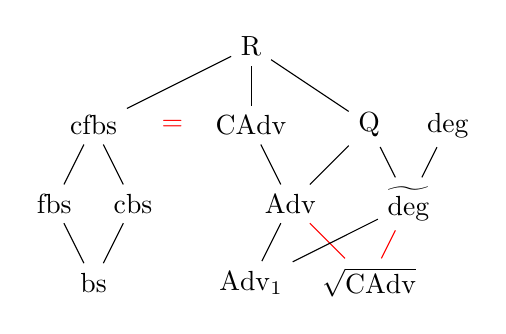
\begin{tikzpicture}[x=0.5cm,y=0.5cm]
     \node (cfbs) at(1,4){$\cfbs$};
     \node (fbs) at(0,2){$\fbs$};
     \node (cbs) at(2,2){$\cbs$};
     \node (bs) at(1,0){$\bs$};
     \node (eq) at(3,4){\color{red}$=$};
     \node (CAdv) at(5,4){$\CAdv$};
     \node (Adv) at(6,2){$\Adv$};
     \node (Advo) at(5,0){$\Adv_1$};
     \node (R) at(5,6){$\R$};
     
     \node (sqCAdv) at(8,0){$\sqrt{\CAdv}$};
     \node (adeg) at(9,2){$\adeg$};
     \node (Q) at(8,4){$\Q$};
     \node (deg) at(10,4){$\deg$};

     \path[-] (sqCAdv) edge[red] (Adv);
     \path[-] (sqCAdv) edge[red] (adeg);
     \path[-] (Adv) edge (Q);
     \path[-] (adeg) edge (Q);
     \path[-] (Q) edge (R);

     \path[-] (bs) edge (cbs);
     \path[-] (bs) edge (fbs);
     \path[-] (fbs) edge (cfbs);
     \path[-] (cbs) edge (cfbs);
     \path[-] (Advo) edge (Adv);
     \path[-] (Advo) edge (adeg);
     \path[-] (Adv) edge (CAdv);
     \path[-] (cfbs) edge (R);
     \path[-] (CAdv) edge (R);
     \path[-] (adeg) edge (deg);
  \end{tikzpicture}
    \caption{Relations between query complexity
    measures used in this work, applicable to partial functions.
    An upwards line from $\M_1(f)$ to $\M_2(f)$ means
    that $\M_1(f)=O(\M_2(f))$ for all (possibly partial) Boolean
    functions $f$. {\color{red}Red} indicates new
    relationships proved in this work.
    We warn that some of these relationships
    are false for relations; in particular, $\CAdv$ may
    be strictly larger than $\cfbs$ and its square root
    may be incomparable to $\adeg$ for relations.
    \label{fig:relations}}
\end{wrapfigure}


It is not hard to see that $\bs(f)$ is the smallest
of the block sensitivity measures, and $\cfbs(f)$ is
the largest. We know \cite{Aar08,HN12}
that $\fbs(f)$ and $\cbs(f)$ both lower bound $\R(f)$
for all (possibly partial) Boolean functions $f$;
in Section 6 of the original publication, we show that $\cfbs(f)$ is also
a lower bound.

We know \cite{LM08,SS06,AKPV18} that
$\Q(f)=\Omega(\Adv(f))$ and $\R(f)=\Omega(\CAdv(f))$.
Although this it not ordinarily stated for relations,
both lower bounds hold when $f$ is a relation as well.
In Section 6 of the original publication, we show that
$\CAdv(f)=\Theta(\cfbs(f))$
for all partial functions $f$,
and we also show that
$\CAdv(f)=O(\Adv(f)^2)$
which holds for both partial functions and relations.

Approximate degree lower bounds quantum query complexity:
$\Q(f)=\Omega(\adeg(f))$.
It is known \cite{BBC+01} that approximate
degree is lower-bounded by $\sqrt{\bs(f)}$.
Tal \cite{Tal13} showed that for total functions,
$\adeg(f)=\Omega(\sqrt{\fbs(f)})$.
In Section 6 of the original publication, we extend this result to partial
functions, and also prove that
$\adeg(f)=\Omega(\sqrt{\cfbs(f)})$.

In conclusion, $\CAdv(f)$ turns out to be the same
as $\cfbs(f)$ for partial functions,
and its square root lower bounds both
$\Adv(f)$ and $\adeg(f)$, both of which are lower bounds
on $\Q(f)$. Without taking square roots,
$\CAdv(f)$ is a lower bound on $\R(f)$
but not on $\Q(f)$.

When we move from partial functions
to relations, the measure $\CAdv(f)$ appears to get stronger
in comparison to the other measures: it is
strictly larger than $\cfbs(f)$, and appears to be
incomparable to $\adeg(f)$ (though defining the
latter for relations is a bit tricky, and we don't
do so in this work).


\subsection{Communication complexity}

In the communication model, two parties, Alice and Bob, are given inputs $x\in\X$ and $y\in\Y$ respectively, and in the most general case the task is to jointly compute a relation $f\subseteq \X\times\Y\times\Z$ by communicating with each other. In other words, on input $(x,y)$,
Alice and Bob must output a symbol
$z\in\Z$ such that $(x,y,z)\in f$.
Without loss of generality, we can assume Alice sends the first message, and Bob produces the output of the protocol.

In the classical randomized model, Alice and Bob are allowed to use shared randomness $R$ (and also possibly private randomness $R_A$ and $R_B$) in order to achieve this. The cost of a communication protocol $\Pi$, denoted by $\CC(\Pi)$ is the number of bits exchanged between Alice and Bob. The randomized communication complexity of a relation $f$ with error $\epsilon$, denoted by $\R^\CC_\epsilon(f)$, is defined as the minimum $\CC(\Pi)$ of a randomized protocol $\Pi$ that computes $f$ with error at most $\epsilon$ on every input.

\paragraph{Classical information complexity.} The information complexity of a protocol with inputs $X,Y$ according to $\mu$, shared randomness $R$ and transcript $\Pi$ is given by
\[ \IC(\Pi,\mu) = I(X:\Pi|YR)_\mu + I(Y:\Pi|XR)_\mu.\]
For any $\mu$ we have, $\IC(\Pi,\mu) \leq \CC(\Pi)$.

\paragraph{} In a quantum protocol $\Pi$, Alice and Bob initially share an entangled state on registers $A_0B_0$, and they get inputs $x$ and $y$ from a distribution $\mu$. The global state at the beginning of the protocol is
\[ \ket{\Psi^0} = \sum_{x,y}\sqrt{\mu(x,y)}\ket{xxyy}_{X\tX Y\tY}\otimes\ket{\Theta^0}_{A_0B_0}\]
where the registers $\tX$ and $\tY$ purify $X$ and $Y$ and are inaccessible to either party. In the $t$-th round of the protocol, if $t$ is odd, Alice applies a unitary $U_t: A'_{t-1}C_{t-1} \to A'_tC_t$, on her input, her memory register $A'_{t-1}$ and the message $C_{t-1}$ from Bob in the previous round (where $A'_0=XA_0$ and $C_0$ is empty), to generate the new message $C_t$, which she sends to Bob, and new memory register $A'_t$. Similarly, if $t$ is even, then Bob applies the unitary $U_t: B'_{t-1}C_{t-1} \to B'_tC_t$ and sends $C_t$ to Alice. It is easy to see that $B'_t=B'_{t-1}$ for odd $t$, and $A'_t=A'_{t-1}$ for even $t$. We can assume that the protocol is safe, i.e., for all $t$, $A'_t=XA_t$ and $B'_t = YB_t$, and $U_t$ uses $X$ or $Y$ only as control registers. The global state at the $t$-th round is then
\[ \ket{\Psi^t} = \sum_{x,y}\sqrt{\mu(x,y)}\ket{xxyy}_{X\tX Y\tY}\otimes\ket{\Theta^t}_{A_tB_tC_t|xy}.\]
\cite{LT17} (Proposition 9) showed that making a protocol safe does not decrease its QIC (defined below), so we shall often work with protocols of this form.

The quantum communication cost of a protocol $\Pi$, denoted by $\QCC(\Pi)$, is the total number of qubits exchanged between Alice and Bob in the protocol, i.e., $\sum_t\log|C_t|$. The quantum communication complexity of $f$ with error $\epsilon$, denoted by $\Q^\CC(f)$, is defined as the minimum $\QCC(\Pi)$ of a quantum protocol $\Pi$ that computes $f$ with error at most $\epsilon$ on every input.

\paragraph{Quantum information complexity.} Given a quantum protocol $\Pi$ as described above with classical inputs distributed as $\mu$, its quantum information complexity is defined as
\[ \QIC(\Pi,\mu) = \sum_{t \text{ odd}}I(\tX\tY:C_t|YB'_t)_{\Psi^t} + \sum_{t\text{ even}}I(\tX\tY:C_t|XA'_t)_{\Psi^t}.\]
The Holevo quantum information complexity is defined as
\begin{align*}
\HQIC(\Pi,\mu) & = \sum_{t\text{ odd}}I(X:B'_tC_t|Y)_{\Psi^t} + \sum_{t\text{ even}}I(Y:A'_tC_t|X)_{\Psi^t} \\
 & = \sum_{t\text{ odd}}I(X:B_tC_t|Y)_{\Psi^t} + \sum_{t\text{ even}}I(Y:A_tC_t|X)_{\Psi^t} \quad \text{(for safe protocols).}
\end{align*}
For brevity, we shall often only use the classical input distribution $\mu$ as the subscript, or drop the subscript entirely, for these information quantities.

It was proved in \cite{LT17}, that for an $r$-round protocol $\Pi^r$, HQIC and QIC satisfy the following relation:
\[ \QIC(\Pi^r, \mu) \geq \frac{1}{r}\HQIC(\Pi^r, \mu) \geq \frac{1}{2r}\QIC(\Pi^r,\mu).\]
Moreover, for any $\mu$, $\QIC(\Pi,\mu) \leq \QCC(\Pi)$.


\section{Lifting the classical adversary}

\subsection{The gadget and its properties}

The gadget we use is the same one used in \cite{GP18},
called \textsc{VER} in that work. This is the function
$\textsc{VER}\colon\B^2\times\B^2\to\B$ defined by $G(x,y)=1$
if and only if $x+y$ is equivalent to $2$ or $3$ modulo $4$,
where $x,y\in\B^2$ are interpreted as binary representations
of integers in $\{0,1,2,3\}$. This gadget has the property
of being \emph{versatile}, which means that it satisfies
the following three properties:
\begin{enumerate}
\item Flippability: given any input $(x,y)$, Alice
and Bob can perform a local operation on their respective inputs (without communicating)
to get $(x',y')$ such that $G(x',y')=1-G(x,y)$.
\item Random self-reducibility: given any input $(x,y)$,
Alice and Bob can use shared randomness (without communicating)
to generate $(x',y')$ which is uniformly distributed over
$G^{-1}(G(x,y))$. That is, Alice and Bob can convert any $0$-input
into a random $0$-input and any $1$-input into a random $1$-input,
without any communication. More formally,
if the domain of $G$ is $\X\times \Y$,
we require a probability distribution $\nu_G$
over pairs of permutations in $S_{\X}\times S_{\Y}$
such that for each $(x,y)\in\X\times\Y$,
sampling $(\sigma_A,\sigma_B)$ from $\nu_G$
and constructing the pair $(\sigma_A(x),\sigma_B(y))$
gives the uniform distribution over $G^{-1}(G(x,y))$.
\item Non-triviality: the function $G$ contains $\AND_2$
as a sub-function (and by flippability, it also contains
$\OR_2$ as a sub-function).
\end{enumerate}

These three properties were established in \cite{GP18} for
the function \textsc{VER}; a gadget which satisfies
them is called \emph{versatile}.
Our lifting proof will work for any versatile gadget $G$.
We will need the following simple lemma, which allows
us to generate $n$-tuples of inputs to $G$ that evaluate
to either a string $s\in\B^n$ or its complement
$\hat{s}\in\B^n$. We use the notation $G^{-1}(s)$
to denote the set of all $n$-tuples of inputs to $G$
that together evaluate to $s\in\B^n$; this abuses
notation slightly (we would technically need to write
$(G^{\oplus n})^{-1}(s)$, where $G^{\oplus n}$ is
the function we get by evaluating $n$ independent inputs
to $G$).

\begin{lemma}\label{lem:s-sampling}
Let $s\in\{0,1\}^m$ be a given string and $G$ be a versatile gadget. Then there is a protocol with no communication using shared randomness between Alice and Bob, who receive inputs $(a,b)$ in the domain of $G$ such that
\begin{itemize}
 \item If $G(a,b)=0$, Alice and Bob produce output strings $(x,y)$ that are uniformly distributed in $G^{-1}(s)$
 \item If $G(a,b)=1$, Alice and Bob produce output strings $(x,y)$ that are uniformly distributed in $G^{-1}(\hat{s}) = G^{-1}(s\oplus1^m)$.
\end{itemize}
\end{lemma}

\begin{proof}
Alice and Bob share independent instances of the permutations $\nu_G$, $\sigma_A$ and $\sigma_B$ as randomness. Applying independent instances of $\nu_G$, Alice and Bob can produce $(x',y')$ that are uniformly distributed in $G^{-1}((G(a,b))^m)$: this is done by applying $m$ independent instances of $\sigma_A$ and $\sigma_B$ from $\nu_G$ to $a$ and $b$ respectively. Now Alice and Bob know where $s$ differs from $0^m$. By applying independent instances of the local flipping operation on $x'$ and $y'$ at these locations, they can negate the output of $G$. It is clear the resultant string $(x,y)$ is uniformly distributed in $G^{-1}(s)$ if $G(a,b)=0$ and in $G^{-1}(\hat{s})$ if $G(a,b)=1$.
\end{proof}

We additionally have the following lemma, which
uses the non-triviality property of a versatile gadget.

\begin{lemma}\label{lem:ANDOR-classical}
If $G$ is a constant-sized non-trivial gadget (containing $\AND_2$ and $\OR_2$ as subfunctions), and $\mu_0$ and 
$\mu_1$ are uniform distributions over its $0$- and $1$-inputs, 
then any classical protocol $\Pi$ for computing $G$ with bounded 
error has $\IC(\Pi,\mu_0), \IC(\Pi,\mu_1) = \Omega(1)$.
\end{lemma}

\begin{proof}
$G$ contains the $\AND_2$ function, and $\mu_0$ puts uniform 
$\Omega(1)$ weight on the 0-inputs of the $\AND_2$ subfunction. 
\cite{BJKS04} showed that any protocol computing the $\AND_2$ 
function must have $\Omega(1)$ information cost with
respect to the distribution that puts
$1/3$ weight on all $0$-inputs of the $\AND_2$ function. Hence any 
protocol for $G$ must also have $\IC(\Pi,\mu_0)=\Omega(1)$. 
Similarly, by considering the fact that $G$ contains the $\OR_2$ 
function, we can show that $\IC(\Pi,\mu_1)=\Omega(1)$.
\end{proof}


Although we only need a single versatile gadget,
such as \textsc{VER}, we will briefly remark that there is
actually an infinite family of versatile gadgets, and that
this family is universal (i.e.\ every communication function
is a sub-function of some gadget in the family).

\begin{lemma}
There is a universal family of versatile gadgets.
\end{lemma}

\begin{proof}
For ease of notation, let $G$ denote \textsc{VER}.
For each $n\in\bN^+$, we define $G_{n}$ to be
$\PARITY_n\circ G$. Note that $G_{n}$ has the signature
$\B^{2n}\times\B^{2n}\to\B$. We observe that $G_{n}$
is versatile for each $n\in\bN^{+}$. This is because,
given a single input $((x_1,x_2,\dots,x_n),(y_1,y_2,\dots,y_n))$
to $G_{n}$ with $x_i,y_i\in\{0,1,2,3\}$ for each $i\in[n]$,
Alice and Bob can locally generate the uniform
distribution over all inputs with the same $G_{n}$-value.
They can do this by first negating a random subset of the
positions $i$ of even size
(using the flippability property of \textsc{VER}),
and then converting each of the $n$ resulting inputs to $G$
into a random input to $G$ with the same $G$-value.

Suppose $z$ is the $n$-bit string with $z_i=G(x_i,y_i)$.
Then flipping a random even subset of the bits of $z$
is equivalent to generating a random string $w$ that has
the same parity as $z$. It follows that the above procedure
generates a random input to $G_{n}$ that has the same $G_{n}$
value as the original input, meaning that $G_{n}$
is random self-reducible. By flipping any single gadget
$G$ within $G_{n}$, we can negate $G_n$, so it is also
flippable. Finally, since $G_n$ contains $G$ as a sub-function,
it also contains $\AND$ as a sub-function, so $G_n$
is versatile for each $n\in\bN^{+}$.

It remains to show that $\{G_n\}_n$ is universal.
We note that since $G$ contains $\AND$ as a sub-function,
and since $G_n=\PARITY_n\circ G$, the function $G_n$
contains $\PARITY_n\circ\AND$ as a sub-function. The latter
is the inner product function $\IP_n$ on $n$ bits,
which is well-known to be universal. Hence $G_n$ is also
universal.
\end{proof}


\subsection{The lifting theorem}

\begin{theorem}
Let $G$ be a constant-sized versatile gadget such as
$\textsc{VER}$, and let $f\colon\B^n\to\Sigma$ be a relation.
Then $\RCC(f\circ G) =\Omega(\CAdv(f))$.
\end{theorem}

\begin{proof}
Let $\Pi$ be a randomized protocol for $f\circ G$ which uses $T$ rounds
of communication (with one bit sent each round), and successfully computes $f\circ G$ with probability at least $1-\epsilon/2$ for each input. Consider inputs $XY$ distributed according to $\mu_z = \mu_{z_1}\otimes\ldots\otimes\mu_{z_n}$, where each $\mu_{z_i}$ is the uniform distribution over $(x_i,y_i)$ in $G^{-1}(z_i)$. Suppose $\Pi$ uses public randomness $R$ which is independent of the inputs $XY$. We introduce the dependency-breaking random variables $D$ and $U$ \cite{BJKS04} in the following way: $D$ is independent of $X, Y, R$ and is uniformly distributed on $\B^n$. For each $i \in [n]$, if $D_i=0$, then $U_i = X_i$, and if $D_i=1$, then $U_i=Y_i$. Defined this way, given $D_iU_i$, $X_i$ and $Y_i$ are independent under $\mu_z$. We shall use this algorithm to give a weight scheme $q'(z,i)$:
\[q'(z,i)=I(X_i:\Pi|X_{<i} YDUR)_{\mu_z} + I(X_i:\Pi|Y_{<i}XDUR)_{\mu_z}\]
where $X_{<i}$ denotes $X_1\ldots X_{i-1}$, and similarly for $Y_{<i}$. Clearly $q$ is non-negative, and we shall show that
\begin{align*}
& \sum_{i:z_i\neq w_i}\min\{q'(z,i),q'(w,i)\} = \Omega(1)
\end{align*}
for all $z,w$ such that $f(z) \cap f(w) = \varnothing$, where the constant in the $\Omega(1)$ is universal. Using this constant to normalize $q'(z,i)$, we get $q(z,i)$ which is a valid weight scheme. Since for any fixed value of $DU=du$, $I(X:\Pi|YR)_{\mu_{zdu}}$ is an information cost,
\[ \sum_{i \in [n]}q'(z,i) = I(X:\Pi|YDUR)_{\mu_z} + I(Y:\Pi|XDUR)_{\mu_z} \leq \CC(\Pi),\]
we have for any protocol $\Pi$,
\[ \CC(\Pi) \geq \Omega\left(\sum_{i \in [n]}q(z,i)\right) \geq \Omega\left(\min_{\{q(z,i)\}}\sum_{i \in [n]}q(z,i)\right) \]
where the minimization is over all valid weight schemes. This proves the result.

Let $z$ and $w$ be two inputs to $f$ such that $f(z) \cap f(w) =\varnothing$. Suppose $z$ and $w$ differ on indices in the block $\cB$. Let $\cB^1$ be the subset of indices in $\cB$ where $\min\{q'(z,i),q'(w,i)\}$ is achieved by $q'(z,i)$, and $\cB^2$ be the subset where the minimum is achieved by $q'(w,i)$. For an index $i\in \cB^1$, let $\cB^1_i$ denote $\cB^1 \cap [i-1]$, and $\cB^2_i$ denote $\cB^2 \cap [i-1]$. We also use $\cB^{1,c}$ to denote $[n]\setminus\cB^1$, and $\cB^{1,c}_i$ to denote $[i-1]\setminus\cB^1_i$. Then,
\begin{align}
&\sum_{i: z_i \neq w_i}\min\left\{q'(z,i), q'(w,i)\right\} \nonumber \\
& = \sum_{i\in \cB^1}(I(X_i:\Pi|X_{<i}YDUR)_{\mu_z} + I(Y_i:\Pi|Y_{<i}XDUR)_{\mu_z}) \nonumber \\
& \quad + \sum_{i\in \cB^2}(I(X_i:\Pi|X_{<i}YDUR)_{\mu_w} + I(Y_i:\Pi|Y_{<i}XDUR)_{\mu_w}) \nonumber \\
& \overset{(1)}= \frac{1}{2}\sum_{i\in \cB^1}(I(X_i:\Pi|X_{<i}YD_{-i}U_{-i}R)_{\mu_z} + I(Y_i:\Pi|Y_{<i}XD_{-i}U_{-i}R)_{\mu_z}) \nonumber \\
& \quad + \frac{1}{2}\sum_{i\in \cB^2}(I(X_i:\Pi|X_{<i}YD_{-i}U_{-i}R)_{\mu_w} + I(Y_i:\Pi|Y_{<i}XD_{-i}U_{-i}R)_{\mu_w}) \nonumber \\
& \overset{(2)}\geq \frac{1}{2}\sum_{i\in \cB^1}(I(X_i:\Pi|X_{\cB^1_i}Y_{\cB^1}D_{\cB^{1,c}}U_{\cB^{1,c}}R)_{\mu_z} + I(Y_i:\Pi|Y_{\cB^1_i}X_{\cB^1}D_{\cB^{1,c}}U_{\cB^{1,c}}R)_{\mu_z}) \nonumber \\
& \quad + \frac{1}{2}\sum_{i\in \cB^2}(I(X_i:\Pi|X_{\cB^2_i}Y_{\cB^2}D_{\cB^{2,c}}U_{\cB^{2,c}}R)_{\mu_w} + I(Y_i:\Pi|Y_{\cB^2_i}X_{\cB^2}D_{\cB^{2,c}}U_{\cB^{2,c}}R)_{\mu_w}) \nonumber \\
& = \frac{1}{2}(I(X_{\cB^1}:\Pi|Y_{\cB^1}D_{\cB^{1,c}}U_{\cB^{1,c}}R)_{\mu_z} + I(Y_{\cB^1}:\Pi|X_{\cB^1}D_{\cB^{1,c}}U_{\cB^{2,c}}R)_{\mu_z}) \nonumber \\
& \quad + \frac{1}{2}(I(X_{\cB^2}:\Pi|Y_{\cB^2}D_{\cB^{2,c}}U_{\cB^{2,c}}R)_{\mu_w} + I(Y_{\cB^2}:\Pi|X_{\cB^2}D_{\cB^{2,c}}U_{\cB^{2,c}}R)_{\mu_w}). \label{inf_ineq}
\end{align}
Above, equality $(1)$ follows by using the definition of $D_iU_i$. The inequality $(2)$ follows from the fact that given $Y_i$, $X_i$ is independent of all other $X_j$-s, $Y_j$-s $D_j$-s and $U_j$-s under both the $z$ and $w$ distributions, hence $I(Y_i:\Pi|Y_{<i}X(DU)_{-i}R)_{\mu_z} \geq I(Y_i:\Pi|Y_{\cB^1_i}X_{\cB^1}(DU)_{\cB^{1,c}}R)_{\mu_z}$, and equivalent inequalities hold for the other terms.

Consider $v \in \{0,1\}^n$ which agrees with $w$ on the bits in $\cB^1$, with $z$ on the bits in $\cB^2$, and with both of them outside $\cB$. Since $f(z)$ and $f(w)$ are disjoint, at least one of the following must be true:
\begin{enumerate}
    \item $\Pr_{(x,y)\sim \mu_v}[\Pi(x,y) \in f(z)] \leq \frac{1}{2}$
    \item $\Pr_{(x,y)\sim \mu_v}[\Pi(x,y) \in f(w)] \leq \frac{1}{2}$.
\end{enumerate}
In case 1, we shall give a protocol $\Pi'$ that computes $G$ correctly with probability at least $1-\epsilon$ in the worst case, such that
\[\IC(\Pi', \mu_0) = O( I(X_{\cB^1}:\Pi|Y_{\cB^1}D_{\cB^{1,c}}U_{\cB^{1,c}}R)_{\mu_z} + I(Y_{\cB^1}:\Pi|X_{\cB^1}D_{\cB^{1,c}}U_{\cB^{1,c}}R)_{\mu_z}).\]
Similarly, in case 2, we can use $\Pi$ to give a protocol $\Pi''$ for $G$, such that
\[ \IC(\Pi'', \mu_1) = O(I(X_{\cB^2}:\Pi|Y_{\cB^2}D_{\cB^{2,c}}U_{\cB^{2,c}}R)_{\mu_w} + I(Y_{\cB^2}:\Pi|X_{\cB^2}D_{\cB^{2,c}}U_{\cB^{2,c}}R)_{\mu_w}).\]
Due to equation \eqref{inf_ineq} and \lem{ANDOR-classical}, this proves the theorem.

In fact we only show how to construct the protocol $\Pi'$ in case 1; the construction of $\Pi''$ is identical. Since $z$ is in the domain of $f$ and $\Pi$ has worst case correctness for $f\circ G$, we must have $\Pr_{(x,y)\sim\mu_z}[\Pi(x,y) \in f(z)] \geq 1-\epsilon/2$. Therefore, in case 1, $\Pi$ can distinguish between samples from $\mu_z$ and $\mu_v$ on average: on getting a sample from $\mu_z$ or $\mu_v$, we can run $\Pi$ to see if it gives an output in $f(z)$ or not, and output $z$ or $v$ accordingly. This average distinguishing probability can be boosted by running $\Pi$ multiple times. 

In $\Pi'$, Alice and Bob will share $RD_{\cB^{1,c}}U_{\cB^{1,c}}R_AR_B$ as randomness, where we use $R_A$ and $R_B$ to denote Alice and Bob's part of the shared randomness from  \lem{s-sampling}, required to generate $z_{\cB^1}$ if $G(a,b)=0$ and $v_{\cB^1}$ if $G(a,b)=1$. On input $(a,b)$ to $G$, Alice and Bob do the following $k$ times for $k=\frac{2}{\epsilon^2}\ln(1/\epsilon)$ :
\begin{itemize}
\item Alice sets $x_{\cB^1} = R_A(a)$ and Bob sets $y_{\cB^1} = R_B(b)$.
\item Alice samples $x_{\cB^{1,c}}$ and Bob samples $y_{\cB^{1,c}}$ from private randomness, so that $G^{|\cB^{1,c}|}(x_{\cB^{1,c}},y_{\cB^{1,c}})$ $= z_{\cB^{1,c}}$. They can do this since given $(DU)_{\cB^{1,c}}$, $X_{\cB^{1,c}}$ and $Y_{\cB^{1,c}}$ are independent under $\mu_z$ and $\mu_v$.
\item They run $\Pi$ on this $(x,y)$ and generate the corresponding output.
\end{itemize}
(There are $k$ independent instances of the $D, U, R_A, R_B$ variables for each run above, but we denote all of them the same way for brevity.) The final output of $\Pi'$ is 1 if the number of runs which have given an output in $f(z)$ is at least $(1-\epsilon)k$, and 0 otherwise.

Clearly if $G(a,b)=0$, then $(x,y)$ generated this way is uniformly distributed in the support of $\mu_z$, and if $G(a,b)=1$, then $(x,y)$ is uniform in the support of $\mu_v$. Calling the protocol in the $i$-th round of $\Pi'$, $\Pi_i$, notice that the transcript of each $\Pi_i$ is independent of $AR_A$, where $A$ is the random variable for Alice's input, given the generated $X_{\cB^1}$ (and this holds true even conditioned on $BR_BD_{\cB^{1,c}}U_{\cB^{1,c}}R$). Moreover, both $X_{\cB^1}$ and $\Pi_i$ are independent of $BR_B$ given $Y_{\cB^1}$ and of $Y_{\cB^1}$ given $BR_B$ (even conditioned on $D_{\cB^1}U_{\cB^1}R$). Let $\mu_{0,z}$ denote the distribution of $ABR_AR_B(DU)_{\cB^{1,c}}$ when $G(a,b)=0$, which induces the distribution $\mu_{z_{\cB^1}}$ on $X_{\cB^1}Y_{\cB^1}$. Hence,
\begin{align*}
I(A:\Pi_i|BR_AR_B(DU)_{\cB^1}R)_{\mu_{0,z}} & \leq I(AR_A:\Pi_i|BR_B(DU)_{\cB^{1,c}}R)_{\mu_{0,z}} \\
 & \overset{(1)}{\leq} I(X_{\cB^1}:\Pi_i|BR_B(DU)_{\cB^{1,c}}R)_{\mu_{0,z}} \\
 & \overset{(2)}{\leq} I(X_{\cB^1}:\Pi_i|Y_{\cB^1}BR_B(DU)_{\cB^{1,c}}R)_{\mu_{0,z}} \\
 & \overset{(3)}{=} I(X_{\cB^1}:\Pi_i|Y_{\cB^1}(DU)_{\cB^{1,c}}R)_{\mu_{0,z}} \\
 & \overset{(4)}{=} I(X_{\cB^1}:\Pi|Y_{\cB^1}(DU)_{\cB^{1,c}}R)_{\mu_z}.
\end{align*}
where inequality (1) follows from the fact that $I(U':V|W) \leq I(U:V|W)$ if $U'$ is independent of $V$ given $UW$, (2) follows from the fact that $I(U:V|W) \leq I(U:V|WW')$ if $V$ is independent of $W'$ given $W$, and (3) follows from $I(U:V|WW')=I(U:V|W')$ if $U$ and $V$ are both independent of $W$ given $W'$. Finally, (4) follows from the definition of $\Pi_i$ and the the fact that the variables $AB$ don't appear in the expression, so we can switch from $\mu_{0,z}$ to $\mu_z$. Similarly,
\[ I(B:\Pi_i|AR_AR_B(DU)_{\cB^{1,c}}R)_{\mu_{0,z_{\cB^1}}} \leq I(Y_{\cB^1}:\Pi|X_{\cB^1}(DU)_{\cB^{1,c}}R)_{\mu_{z_{\cB^1}}},\]
which lets us conclude that
\[\IC(\Pi_i,\mu_0) \leq I(X_{\cB^1}:\Pi|Y_{\cB^1}(DU)_{\cB^{1,c}}R)_{\mu_z} + I(Y_{\cB^1}:\Pi|X_{\cB^1}(DU)_{\cB^{1,c}}R)_{\mu_z}.\]
The final $\IC(\Pi',\mu_0)$ is then at most $k(I(X_{\cB^1}:\Pi|Y_{\cB^1}(DU)_{\cB^{1,c}}R)_{\mu_z} + I(Y_{\cB^1}:\Pi|X_{\cB^1}(DU)_{\cB^{1,c}}R)_{\mu_z})$.

Now let us analyze the worst case error made by $\Pi'$. Since the output of $\Pi_i$ on $(a,b)$ is expected output of $\Pi$ on $(x,y)$ uniformly sampled from either $\mu_z$ or $\mu_v$, $\Pi_i$ produces an output in $f(z)$ on $(a,b)$ such that $G(a,b)=0$ with probability at least $1-\epsilon/2$, and on $(a,b)$ such that $G(a,b)=1$ with probability at most $\frac{1}{2}$. Hence by the Hoeffding bound, the probability of $(1-\epsilon)k$ many 0 outputs in the first case is at least
\[ 1-e^{-\epsilon^2k/2} \geq 1- \epsilon\]
and in the second case is at most
\[ e^{-2(1/2-\epsilon)^2k} \leq \epsilon.\]
Hence the probability of error on either input is at most $\epsilon$.
\end{proof}



\begin{thebibliography}{99}
\bibitem{Aar06} Scott Aaronson Lower Bounds for Local Search by Quantum Arguments {SIAM} Journal on Computing 35 4 804-- 824 2006.
\bibitem{Aar08} Scott Aaronson Quantum certificate complexity Journal of Computer and System Sciences 74 3 313-- 322 2008.
\bibitem{ABK+20} Scott Aaronson, Shalev Ben-David, Robin Kothari, Shravas Rao, Avishay Tal Degree vs. Approximate Degree and Quantum Implications of Huang's Sensitivity Theorem 2020.
\bibitem{AF04} R Alicki, M Fannes Continuity of quantum conditional information Journal of Physics A: Mathematical and General 37 5 L55-- L57 2004.
\bibitem{AKPV18} Andris Ambainis, Martins Kokainis, Kri{š}j{ā}nis Pr{ū}sis, Jevg{ē}nijs Vihrovs All Classical Adversary Methods are Equivalent for Total Functions Proceedings in the 35th Symposium on Theoretical Aspects of Computer Science ({STACS}) 2018.
\bibitem{Amb02} Andris Ambainis Quantum Lower Bounds by Quantum Arguments Journal of Computer and System Sciences 64 4 750-- 767 2002.
\bibitem{BBC+01} Robert Beals, Harry Buhrman, Richard Cleve, Michele Mosca, Ronald De~ Wolf Quantum lower bounds by polynomials Journal of the {ACM} 48 4 778-- 797 2001.
\bibitem{BJKS04} Ziv Bar-Yossef, T.S. Jayram, Ravi Kumar, D. Sivakumar An information statistics approach to data stream and communication complexity Journal of Computer and System Sciences 68 4 702-- 732 2004.
\bibitem{BdW02} Harry Buhrman, Ronald Wolf Complexity measures and decision tree complexity: a survey Theoretical Computer Science 288 1 21-- 43 2002.
\bibitem{GP18} Mika Göös, Toniann Pitassi Communication Lower Bounds via Critical Block Sensitivity {SIAM} Journal on Computing 47 5 1778-- 1806 2018.
\bibitem{HN12} Trinh Huynh, Jakob Nordstrom On the virtue of succinct proofs Proceedings of the 44th Annual {ACM} {SIGACT} Symposium on Theory of Computing ({STOC}) 2012.
\bibitem{KT16} Raghav Kulkarni, Avishay Tal On Fractional Block Sensitivity Chicago Journal of Theoretical Computer Science 2016.
\bibitem{LM08} Sophie Laplante, Frédéric Magniez Lower bounds for randomized and quantum query complexity using {K}olmogorov arguments {SIAM} Journal on Computing 2008.
\bibitem{LT17} Mathieu Laurière, Dave Touchette The Flow of Information in Interactive Quantum Protocols: the Cost of Forgetting Proceedings of the 8th Innovations in Theoretical Computer Science Conference ({ITCS}) 2017.
\bibitem{Nis91} Noam Nisan CREW PRAMs and decision trees {SIAM} Journal on Computing 20 6 999-- 1007 1991.
\bibitem{SS06} Robert {Š}palek, Mario Szegedy All Quantum Adversary Methods are Equivalent Theory of Computing 2 2006.
\bibitem{Tal13} Avishay Tal Properties and Applications of Boolean Function Composition Proceedings of the 4th Innovations in Theoretical Computer Science Conference ({ITCS}) 441-- 454 2013.
\end{thebibliography}
\end{document}
